\documentclass[conference]{IEEEtran}

\usepackage{subcaption,graphicx,url,times,multirow,amsmath,amssymb,algorithm,xspace,epsfig,todonotes,array,caption,color}
\hyphenation{op-tical net-works semi-conduc-tor IEEEtran des-cri-bed}
\usepackage{float}
\usepackage[noend]{algpseudocode}
\usepackage[bookmarks=false]{hyperref}


%\IEEEoverridecommandlockouts

\newcommand{\TODO}[2]{\textcolor{#1}{#2}}
\definecolor{red}{RGB}{255,0,0}
\newcommand{\vect}[1]{\boldsymbol{#1}}
\providecommand{\e}[1]{\ensuremath{\times 10^{#1}}}
\DeclareMathOperator*{\argmax}{arg\,max}


\newenvironment{mitems}
{\begin{itemize}
\setlength{\itemsep}{1pt}
\setlength{\parskip}{0pt}
\setlength{\parsep}{0pt}}{\end{itemize}}

\newcommand{\twopartdef}[4]
{
  \left\{
    \begin{array}{ll}
      #1 & \mbox{if } #2 \\
      #3 & \mbox{if } #4
    \end{array}
  \right.
}

\newcommand{\twopartdefo}[3]
{
  \left\{
    \begin{array}{ll}
      #1 & \mbox{if } #2 \\
      #3 & \mbox{otherwise}
    \end{array}
  \right.
}


% correct bad hyphenation here
\hyphenation{op-tical net-works semi-conduc-tor}


\begin{document}
%
% paper title
% can use linebreaks \\ within to get better formatting as desired
\title{Neuroevolution for General Video Game Playing}

\author{\IEEEauthorblockN{Spyridon Samothrakis, Diego Perez-Liebana, Simon M. Lucas and Maria Fasli}
\IEEEauthorblockA{School of Computer Science and Electronic Engineering\\
University of Essex, Colchester CO4 3SQ, UK\\
ssamot@essex.ac.uk, dperez@essex.ac.uk, sml@essex.ac.uk, mfasli@essex.ac.uk}
}


% make the title area
\maketitle


\begin{abstract}
%\boldmath
General Video Game Playing (GVGP) allows for the fair evaluation of algorithms and agents as it minimizes the ability of an agent to exploit apriori knowledge in the form of game specific heuristics. In this paper we compare four possible combinations of evolutionary learning using Separable Natural Evolution Strategies as our evolutionary algorithm of choice; linear function approximation with \textit{Softmax} search and $\epsilon$-\textit{greedy} policies and neural networks with the same policies. The algorithms explored in this research play each of the games during a sequence of $1000$ matches, where the score obtained is used as a measurement of performance. We show that learning is achieved in $8$ out of the $10$ games employed in this research, without introducing any domain specific knowledge, leading the algorithms to maximize the average score as the number of games played increases.

\end{abstract}

\IEEEpeerreviewmaketitle

\section{Introduction} \label{sec:intro}

Learning how to act in unknown environments is often termed the ``Reinforcement Learning'' problem~\cite{sutton1998introduction}. The problem encapsulates the core of artificial intelligence and has been studied widely under different contexts. Broadly speaking, an agents tries to maximize some long term notion of utility or reward by selecting appropriate actions at each state. Classic RL assumes that state can somehow be identified by the agent in a unique fashion, but it is often the case that function approximators are used to help with state spaces that cannot be enumerated. 

A possible way of attacking the problem in the general sense is Neuroevolution (for an example in games see ~\cite{stanley2005real}). Neuroevolution adapts the weights of a local or global function approximator (in the form of a neural network) in order to maximize reward. The appeal of Neurovolution over traditional gradient-based Reinforcement Learning methods is three-fold. First, the gradient in RL problems might be unstable and/or hard to approximate, thus requiring extensive hyper-parameter tuning in order to get any performance. Secondly, the tournament-ranking schemes used by evolutionary approaches are robust to outliers, as they are effectively calculations of medians rather than means. Thirdly, classic RL algorithms (at least their critic-only versions~\cite{singh1994learning}) can be greatly impacted by the lack of a perfect Markov state. Sensor aliasing is a known and common problem in RL under function approximation. 

On one hand, the lack of direct gradient information limits the possible size of the parameters of the function approximator to be evolved. If provided with the correct setup and hyperparameters, RL algorithms might be able to perform at superhuman level in a number of hard problems. In practical terms, research into RL has often been coupled with the use of strong heuristics. General Game Playing allows for completely arbitrary games, making the easy application of temporal based methods non-trivial. On the other hand, modern evolutionary algorithms require minimum fine-tuning and can help greatly with providing a quick baseline. In this paper we perform experiments using evolutionary algorithms to learn actors in the following setup. 

Among evolutionary algorithms, for problems with continuous state variables,  a simple yet robust algorithm is Separable Natural Evolution Strategies (S-NES)~\cite{schaul2011high}. Coupling the algorithm with different policy schemes and different approximators yields the experimental methods: 

\begin{mitems}
\item S-NES using e-greedy policy and a linear function approximator. 
\item S-NES using e-greedy policy and a neural network.
\item S-NES using softmax policy and a linear function approximator.
\item S-NES using softmax policy and a neural network.
\end{mitems}

The motivation behind this is to check whether there is an exploration method which works better in a general sense, without misguiding the evolution. We will see specifics of this setup in later sections. In order to make this research easy to replicate and interesting in its own right, the environmental substrate is provided by the new track of the General Video Game Playing AI Competition\footnote{\url{www.gvgai.net}}. The players evaluated in this research are tested in this setup.

The paper is structured as follows: Section \ref{sec:lit} does a brief review of the current state of the art in General Game and Video Game Playing. Section ~\ref{sec:framework} analyses the framework used in this paper for evaluating games. We describe the algorithms used in Section~\ref{sec:approaches}, while in Section~\ref{sec:exp} we present the experimental results. We conclude with a discussion in Section~\ref{sec:conc}. 
 
\section{Related Research} \label{sec:lit}

While there has been considerable research in the topic of both Neuroevolution and General Game Playing (GGP), GGP~\cite{genesereth2005general} was initially mostly concerned with approaches that included access to a forward model. In this scenario, agents (or players) have the ability to predict the future to a certain extent and plan their actions, typically in domains that are more closely aligned to board games and are of a deterministic nature.

Recently, a competition termed ``The General Video Game Playing Competition''~\cite{Perez2015} has focused on similar problems, but this time in the real-time game domain. The competition provided the competitors with internal models they could sample from (but not access to specific future event probabilities), while limiting the amount of ``thinking'' time provided for an agent to $40$ms (imposing an-almost-real-time constraint). In both contexts, the algorithms that dominated were sample based search methods~\cite{finnsson2008simulation, Perez2015}, also known as Monte Carlo Tree Search (MCTS). In the case of GVG-AI~\cite{Perez2015}, which allows for stochastic environments, Open Loop MCTS methods seem to perform best. A recent paper studies the use of open loop methods, employing both tree search and evolutionary algorithms, in this domain~\cite{Perez2015a}.

This competition and framework has brought more research in this area during the last months, after the end of the contest. For instance, B. Ross, in his Master thesis~\cite{Ross2014}, explores enhancements to the short-sight of MCTS in this domain by adding a long term goal based approach. Also recently, T. Nielsen et al.~\cite{Nielsen2015} employed different game playing algorithms to identify well and badly designed games, under the assumption that good games should differentiate well the performance of these different agents.

There has also been considerable effort in learning how to play games in a generic fashion outside competitions,  using the Atari framework~\cite{13jair}, which provides a multitude of games for testing. The games were tackled recently~\cite{mnih2015human} using a combination of neural networks and Q-learning with experience replay. The method was widely seen as a success (though it could still not outperform humans in all games). The methods for these games operate on a pixel level and require a significant amount of training, but the results achieved when successful cover the full AI loop (from vision to actions). 

This latest work (by Mihn et al.) is of special interest to this research, as it tackles the problem in a similar way to how it is done here. The agents that play those games have no access to a forward model that allows them to anticipate the state that will be found after applying an action. Learning is performed by maximizing the score obtained in the games after playing them during a number of consecutive trials. 

Neuroevolution has been used for real time video games~\cite{stanley2005real},  General Game Playing (see~\cite{reisinger2007coevolving}) and playing Atari games~\cite{hausknecht2012hyperneat, hausknecht2014neuroevolution}, all with varying degrees of success. In the front of solving Atari games, neuroevolution showed strong results using HyperNEAT~\cite{gauci2010autonomous}, a method that evolves all network parameters, including the topology of the network. 

Note that the approach taken herein has the goal of just creating a baseline, not to create competitive agents. It is an ad-hoc method for neurovolution with very limited time and almost no feature engineering. If however one dedicates the right effort and fine tunes enough, we expect Reinforcement Learning (e.g., Q-learning) approaches to outperform the current set of agents. 



\section{The GVGAI Framework} \label{sec:framework}


\subsection{The framework} \label{ssec:framework}

The General Video Game Playing competition and framework (GVG-AI) is built on VGDL (Video Game Description Language), a framework designed by Ebner et al.~\cite{Ebner2013} and developed by T. Schaul~\cite{schaul2013pyvgdl} for GVGP in Python (\textit{py-vgdl}). In VGDL, there are several \textit{objects} that interact in a two-dimensional rectangular space, with associated coordinates and with the possibility of moving and colliding with each other. VGDL defines an ontology that allows the generation of real-time games and levels with simple text files.

The GVG-AI framework is a Java port of py-vgdl, re-engineered for the GVG-AI Competition by Perez et al.~\cite{Perez2015}, which exposes an interface that allows the implementation of controllers that must determine the actions of the player (also referred to as the \textit{avatar}). The VGDL definition of the game is \textbf{not} provided, so it is the responsibility of the agent to determine the nature of the game and the actions needed to achieve victory. 

The original version of this framework provided a \textit{forward model}, that allowed the agent to simulate actions on the current state to devise the consequences of the available actions. In this case, the agents counted on $40ms$ of CPU time to decide an action on each game cycle. This version of the framework was employed by the organizers of the competition to run what is now called the ``planning track'' of the contest, which took part during the Computational Intelligence in Games (CIG) conference in Dortmund (Germany) in 2014. A complete description of this competition, framework, rules, entries and results have been published in~\cite{Perez2015}.

2016 will feature a new track for this competition, named ``learning track''. In this track, controllers do \textbf{not} have access to a forward model, so they cannot foresee the states reached after applying any of the available actions of the game. In contrast, they will be offered the possibility of playing the game multiple times, with the aim of allowing the agents to learn how to play each given game. Note that the competition is not limited by some of the drawbacks related to using Atari as an approach (e.g., no true stochasticity~\cite{hausknecht2015impact}) and that it allows for games that can be customised easily, and also allows for great flexibility in the choice of interface between the game andthe AI agent, which could be vision based (as with ALE) or game-object based (as with the current experiments). Thus, we think, it provides different challenges than Atari General Game Playing. 

Information is given regarding the state of the game to the controllers at three different stages: at initialization, each game step (\textit{act} call, called repeatedly, until the game is finished) and at termination. Table~\ref{tab:inf} summarizes the information given to the agent and at which stages this is passed.


\begin{table*}[!t]
\begin{center}
\begin{tabular}{|m{2.85cm}|m{5cm}|m{5.25cm}|m{0.4cm}|m{0.4cm}|m{0.4cm}|}
%\begin{tabular}{|c|c|c|c|c|c|}
\hline
\textbf{Information}  & \textbf{Description} & \textbf{Possible Values} &  \textbf{Init} &  \textbf{Act} &  \textbf{End} \\ 
\hline
\multicolumn{6}{|c|}{\textbf{Game Information}} \\
\hline
\textbf{Score} & Score of the game. & $[0 .. N] \in \mathbb{N}$ & \checkmark & \checkmark & \checkmark \\
\hline
\textbf{Game tick} & Current game tick. & $[0 .. 1000] \in \mathbb{N}$ & \checkmark & \checkmark & \checkmark \\
\hline
\textbf{Game winner} & Indicates the result of the game for the player. & $\left \{ won, lost, ongoing \right \}$ & \checkmark & \checkmark & \checkmark \\
\hline
\textbf{Is game over} & Indicates if the game is over. & $\left \{ true, false \right \}$ & \checkmark & \checkmark & \checkmark \\
\hline
\textbf{World's dimension (width)} & Width of the level (in pixels). & $[0 .. N] \in \mathbb{R}$ & \checkmark &  &   \\
\hline
\textbf{World's dimension (height)} & Height of the level (in pixels). & $[0 .. N] \in \mathbb{R}$ & \checkmark &  &   \\
\hline
\textbf{Block size (\textit{bs})} & Number of pixels each grid cell has. & $[0 .. N] \in \mathbb{N}$ & \checkmark &  &   \\
\hline
\multicolumn{6}{|c|}{\textbf{Actions Information}} \\
\hline
\textbf{Actions} & Available actions of the game. & A subset of $\left \{ nil, up, down, left, right, use \right \}$ & \checkmark &  &   \\
\hline
\multicolumn{6}{|c|}{\textbf{Avatar Information}} \\
\hline
\textbf{Avatar position ($x$)} & $x$ coordinate (in pixels) of the avatar's position. & $[0 .. N] \in \mathbb{R}$ & \checkmark &  \checkmark  & \checkmark  \\
\hline
\textbf{Avatar position ($y$)} & $y$ coordinate (in pixels) of the avatar's position. & $[0 .. N] \in \mathbb{R}$ & \checkmark & \checkmark & \checkmark  \\
\hline
\textbf{Avatar orientation ($x$)} & $x$ coordinate of the avatar's orientation. & $\left \{ -1, 0, 1 \right \}$ & \checkmark & \checkmark &  \checkmark \\
\hline
\textbf{Avatar orientation ($y$)} & $y$ coordinate of the avatar's orientation.. & $\left \{ -1, 0, 1 \right \}$ & \checkmark & \checkmark & \checkmark  \\
\hline
\textbf{Avatar speed} & Speed of the avatar (pixels/tick). & $[0 .. N] \in \mathbb{N}$ & \checkmark & \checkmark & \checkmark  \\
\hline
\textbf{Avatar last action} & Last action played by the avatar. & One of $\left \{ nil, up, down, left, right, use \right \}$  & \checkmark & \checkmark & \checkmark  \\
\hline
\textbf{Avatar resources} & Collections of pairs $<K,V>$, where $K$ is the type of resource and $V$ is the amount owned. & $\left \{ <K_1,V_1>, <K_2,V_2>, ... \right \}; K_i ,V_i \in \mathbb{N}$  & \checkmark & \checkmark & \checkmark  \\
\hline
\multicolumn{6}{|c|}{\textbf{Grid Information (for each type of sprite)}} \\
\hline
\textbf{Sprite type} & Sprite identifier.& $[0 .. N] \in \mathbb{N}$ & \checkmark & \checkmark & \checkmark  \\
\hline
\textbf{Grid Bitmap} & Presence array of the sprite type on the grid. \newline $1$ means presence, $0$ means absence. & Array $\left \{ 0, 1 \right \}$ of size $[width/bs, height/bs]$ & \checkmark & \checkmark & \checkmark  \\
\hline
\end{tabular}
\caption{Information given to the controllers for action decision. The controller of the agent receives this information on the three different calls: \textit{Init} (at the beginning of the game), \textit{Act} (at every game cycle) and \textit{End} (when the game is over). Pieces of information that are only sent on the \textit{Init} call are constant throughout the game played.}
\label{tab:inf}
\end{center}
\end{table*}


\subsection{Games} \label{ssec:games}

The games employed for this research are the ones from the training set of the GVG-AI competition. These games are described in detail here: 

\subsubsection{Aliens} Similar to traditional Space Invaders, Aliens features the player (avatar) at the bottom of the screen, shooting upwards at aliens that approach Earth, who also shoot back at the avatar. The player loses if any alien touches it, and wins if all the aliens are eliminated. \textit{Scoring:} $1$ point is awarded for each alien or protective structure destroyed by the avatar, and $-1$ point is given if the player is hit. 

\subsubsection{Boulderdash} The avatar must dig in a cave to find at least $10$ diamonds, with the aid of a shovel, before exiting through a door. Some heavy rocks may fall while digging, killing the player if it is hit from above. There are enemies in the cave that might kill the player, but if two different enemies collide, a new diamond is spawned. \textit{Scoring:} $2$ points are awarded for each diamond collected, and $1$ point every time a new diamond is spawned. Also, $-1$ point is given if the avatar is killed by a rock or an enemy.

\subsubsection{Butterflies} The avatar must capture butterflies that move randomly around the level. If a butterfly touches a cocoon, more butterflies are spawned. The player wins if it collects all butterflies, but loses if all cocoons are opened. \textit{Scoring:} $2$ points are awarded for each butterfly captured. 

\subsubsection{Chase} The avatar must chase and kill scared goats that flee from the player. If a goat finds another goat's corpse, it becomes angry and chases the player. The player wins if all scared goats are dead, but it loses if is hit by an angry goat. \textit{Scoring:} $1$ point for killing a goat and $-1$ point for being hit by an angry goat.

\subsubsection{Frogs} The avatar is a frog that must cross a road full of tracks and a river, only traversable by logs, to reach a goal.  The player wins if the goal is reached, but loses if it is hit by a truck or falls into the water. \textit{Scoring:}  $1$ point for reaching the goal, and $-2$ points for being hit by a truck.

\subsubsection{Missile Command} The avatar must shoot at several missiles that fall from the sky before they reach the cities they are directed towards. The player wins if it is able to save at least one city, and loses if all cities are hit. \textit{Scoring:} $2$ points are given for destroying a missile and $-1$ point for each city hit.

\subsubsection{Portals} The avatar must find the goal while avoiding lasers that kill it. There are many portals that teleport the player from one location to another. The player wins if the goal is reached, and loses if killed by a laser.        
 \textit{Scoring:} $1$ point is given for reaching the goal. 

\subsubsection{Sokoban} The avatar must push boxes so they fall into holes. The player wins if all boxes are made to disappear, and loses when the timer runs out. \textit{Scoring:} $1$ point is given for each box pushed into a hole. 

\subsubsection{Survive Zombies} The avatar must stay alive while being attacked by spawned zombies. It may collect honey, dropped by bees, in order to avoid being killed by zombies. The player wins if the timer runs out, and loses if hit by a zombie while having no honey (otherwise, the zombie dies). \textit{Scoring:} $1$ point is given for collecting one piece of honey, and also for killing a zombie. Additionally, $-1$ point if the avatar is killed or it falls into the zombie spawn point.

\subsubsection{Zelda} The avatar must find a key in a maze to open a door and exit. The player is also equipped with a sword to kill enemies existing in the maze. The player wins if it exits the maze, and loses if it is hit by an enemy. \textit{Scoring:} $2$ points for killing an enemy, $1$ for collecting the key, and another point for reaching the door with it. $-1$ point is given if the avatar is killed. 


%\begin{table*}[!t]
%\begin{center}
%\begin{tabular}{|m{1.4cm}|m{8cm}|m{6cm}|}
%\hline
%\textbf{Game}  & \textbf{Description} & \textbf{Score} \\ 
%\hline
%\textbf{Aliens} & Similar to traditional Space Invaders, Aliens features the player (avatar) in the bottom of the screen, shooting upwards at aliens that approach Earth, who also shoot back at the avatar. The player loses if any alien touches it, and wins if all aliens are eliminated. & \begin{list}{$\bullet$}{\leftmargin=2pt \itemindent=0em} \item $1$ point is awarded for each alien or protective structure destroyed by the avatar. \item $-1$ point is given if the player is hit. \end{list} \\
%\hline
%\textbf{Boulderdash} & The avatar must dig in a cave to find at least $10$ diamonds, with the aid of a shovel, before exiting through a door. Some heavy rocks may fall while digging, killing the player if it is hit from above. There are enemies in the cave that might kill the player, but if two different enemies collide, a new diamond is spawned.& \begin{list}{$\bullet$}{\leftmargin=2pt \itemindent=0em} \item $2$ points are awarded for each diamond collected, and $1$ point every time a new diamond is spawned. \item $-1$ point is given if the avatar is killed by a rock or an enemy. \end{list} \\
%\hline
%\textbf{Butterflies} & The avatar must capture butterflies that move randomly around the level. If a butterfly touches a cocoon, more butterflies are spawned. The player wins if it collects all butterflies, but loses if all cocoons are opened. & \begin{list}{$\bullet$}{\leftmargin=2pt \itemindent=0em} \item $2$ points are awarded for each butterfly captured. \end{list} \\
%\hline
%\textbf{Chase} & The avatar must chase and kill scared goats that flee from the player. If a goat finds another goat's corpse, it becomes angry and chases the player. The player wins if all scared goats are dead, but it loses if is hit by an angry goat. & \begin{list}{$\bullet$}{\leftmargin=2pt \itemindent=0em} \item $1$ point for killing a goat. \item $-1$ point for being hit by an angry goat. \end{list} \\
%\hline
%\textbf{Frogs} & The avatar is a frog that must cross a road, full of tracks, and a river, only traversable by logs, to reach a goal.  The player wins if the goal is reached, but loses if it is hit by a truck or falls into the water. & \begin{list}{$\bullet$}{\leftmargin=2pt \itemindent=0em} \item $1$ point for reaching the goal. \item $-2$ points for being hit by a truck. \end{list} \\
%\hline
%\textbf{Missile Command} & The avatar must shoot at several missiles that fall from the sky, before they reach the cities they are directed towards. The player wins if it is able to save at least one city, and loses if all cities are hit. &  \begin{list}{$\bullet$}{\leftmargin=2pt \itemindent=0em} \item $2$ points are given for destroying a missile. \item $-1$ point for each city hit. \end{list} \\
%\hline
%\textbf{Portals} & The avatar must find the goal while avoiding lasers that kill him. There are many portals that teleport the player from one location to another. The player wins if the goal is reached, and loses if killed by a laser.& \begin{list}{$\bullet$}{\leftmargin=2pt \itemindent=0em} \item $1$ point is given for reaching the goal. \end{list} \\
%\hline
%\textbf{Sokoban} & The avatar must push boxes so they fall into holes. The player wins if all boxes are made to disappear, and loses when the timer runs out. & \begin{list}{$\bullet$}{\leftmargin=2pt \itemindent=0em} \item $1$ point is given for each box pushed into a hole. \end{list} \\
%\hline
%\textbf{Survive Zombies} & The avatar must stay alive while being attacked by spawned zombies. It may collect honey, dropped by bees, in order to avoid being killed by zombies. The player wins if the timer runs out, and loses if hit by a zombie while having no honey (otherwise, the zombie dies).& \begin{list}{$\bullet$}{\leftmargin=2pt \itemindent=0em} \item $1$ point is given for collecting one piece of honey, and also for killing a zombie. \item $-1$ point if the avatar is killed, or it falls into the zombie spawn point. \end{list} \\
%\hline
%\textbf{Zelda} & The avatar must find a key in a maze to open a door and exit. The player is also equipped with a sword to kill enemies existing in the maze. The player wins if it exits the maze, and loses if it is hit by an enemy. & \begin{list}{$\bullet$}{\leftmargin=2pt \itemindent=0em} \item $2$ points for killing an enemy, $1$ for collecting the key, and another point for reaching the door with it. \item $-1$ point if the avatar is killed. \end{list} \\
%\hline
%\end{tabular}
%\caption{Games in the training set of the GVGAI Competition, employed in the experiments of this paper.}
%\label{tab:games}
%\end{center}
%\end{table*}

In order to show the diversity of these games, Table~\ref{tab:gamesComparative} shows the features of each one of them. In this table, the \texttt{Score System} indicates how the reward is given to the avatar by means of a numeric score. This system can be either \textbf{binary} (B) or \textbf{incremental} (I). In the former case, the score of the game will always be $0$ until victory is achieved, when the reward will become $1$. In the latter scenario, points are regularly awarded throughout the course of the game.

\begin{table*}[!t]
\begin{center}
\begin{tabular}{|c|c|c|c|c|c|c|c|c|c|}
\hline
\multirow{2}{*}{\textbf{Game}} & \multirow{2}{*}{\textbf{Score System}} & \multicolumn{3}{c|}{\textbf{NPC Types}} & \multirow{2}{*}{\textbf{Resouces}} & \multicolumn{3}{c|}{\textbf{Terminations}} & \multirow{2}{*}{\textbf{Action Set}}\\ 
\cline{3-5}
 \cline{7-9}
 &  &  Friendly & Enemies & $>1$ type & & Counters & Exit Door & Timeout & \\
 
\hline
\hline
\textbf{Aliens} & I &  & \checkmark &  &  & \checkmark &  & & A2\\
\hline
\textbf{Boulderdash} & I  &  & \checkmark & \checkmark & \checkmark &  & \checkmark & & A0\\
\hline
\textbf{Butterflies} & I & \checkmark &  &  &  & \checkmark &  & & A1\\
\hline
\textbf{Chase} & I & \checkmark & \checkmark &  &  & \checkmark &  & & A1\\
\hline
\textbf{Frogs} & B  &  &  &  &  &  & \checkmark & & A1\\
\hline
\textbf{Missile Command} & I  &  & \checkmark &  &  & \checkmark &  & & A0\\
\hline
\textbf{Portals} & B  &  &  &  &  &  & \checkmark & & A1\\
\hline
\textbf{Sokoban} & I  &  &  &  &  & \checkmark &  & & A1\\
\hline
\textbf{Survive Zombies} & I  & \checkmark & \checkmark &  & \checkmark &  &  & \checkmark & A1\\
\hline
\textbf{Zelda} & I &  & \checkmark &  & \checkmark &  & \checkmark &  & A0\\
\hline
\end{tabular}
\caption{Games feature comparative, showing all games employed in this study.  Legend: I: Incremental; B: Binary; A0: All moves; A1: Only directional; A2: Left, right
and use. Check Section III-B for a full description of the meaning of all terms in this table.}
\label{tab:gamesComparative}
\end{center}
\end{table*}


The second column, \texttt{NPC Types}, indicates the sort of other moving entities that can be found in the game. \textit{Friendly} refers to the Non Player Characters (NPC) that do not harm the player, whereas \textit{Enemies} refer to those NPCs that pose some hazard in the game. Additionally, one game also features more than one type of enemy (\textit{Boulderdash}).

\texttt{Resources} indicates if the game contains sprites that can be picked up by the player or not, and \texttt{Terminations} relates to how the game can end. A game can finish either by creating or destroying one or more sprites of a given type (column \textit{Counters}), reaching a goal (\textit{Exit Door}) or when a timer runs out (\textit{Timeout}). Independently, all games can finish eventually (with a loss) it the maximum number of game steps that can be played, set to $1000$ for all games, is reached. This limit is introduced in order to avoid degenerate players from never finishing the game.

Finally, each one of these games provides a different set of available actions to the player. The games labelled in Table~\ref{tab:gamesComparative} as $a0$ provide the complete set of actions ($\left \{ nil, up, down, left, right, use \right \}$). $A1$ games are those where the actions are only directional (this is, the complete set without the $use$ action). Finally, $A2$ indicates the subset composed by $\left \{ nil, left, right, use \right \}$.

It is worthwhile highlighting that the variety of these games poses a serious hazard to the playing agents. The learning algorithm needs to learn how the game has to be played in order to achieve victory and maximize score. It is important to realize that the description of the game is not passed to the agent at any time, thus the only way the agent can learn how to play the game is to analyze the game state (maybe by extracting features) and build relations between the observations and the games played.

Of course, one could try to identify the game that is being played and act consequently. However, this is of a limited research interest, as the long term objective is to find agents that can learn any game (rather than building an agent that uses a database of known games, heuristically prepared to play these).  Figure~\ref{fig:games} shows screenshots of four of the games employed in this research.

\begin{figure*}[!t]
\begin{center}
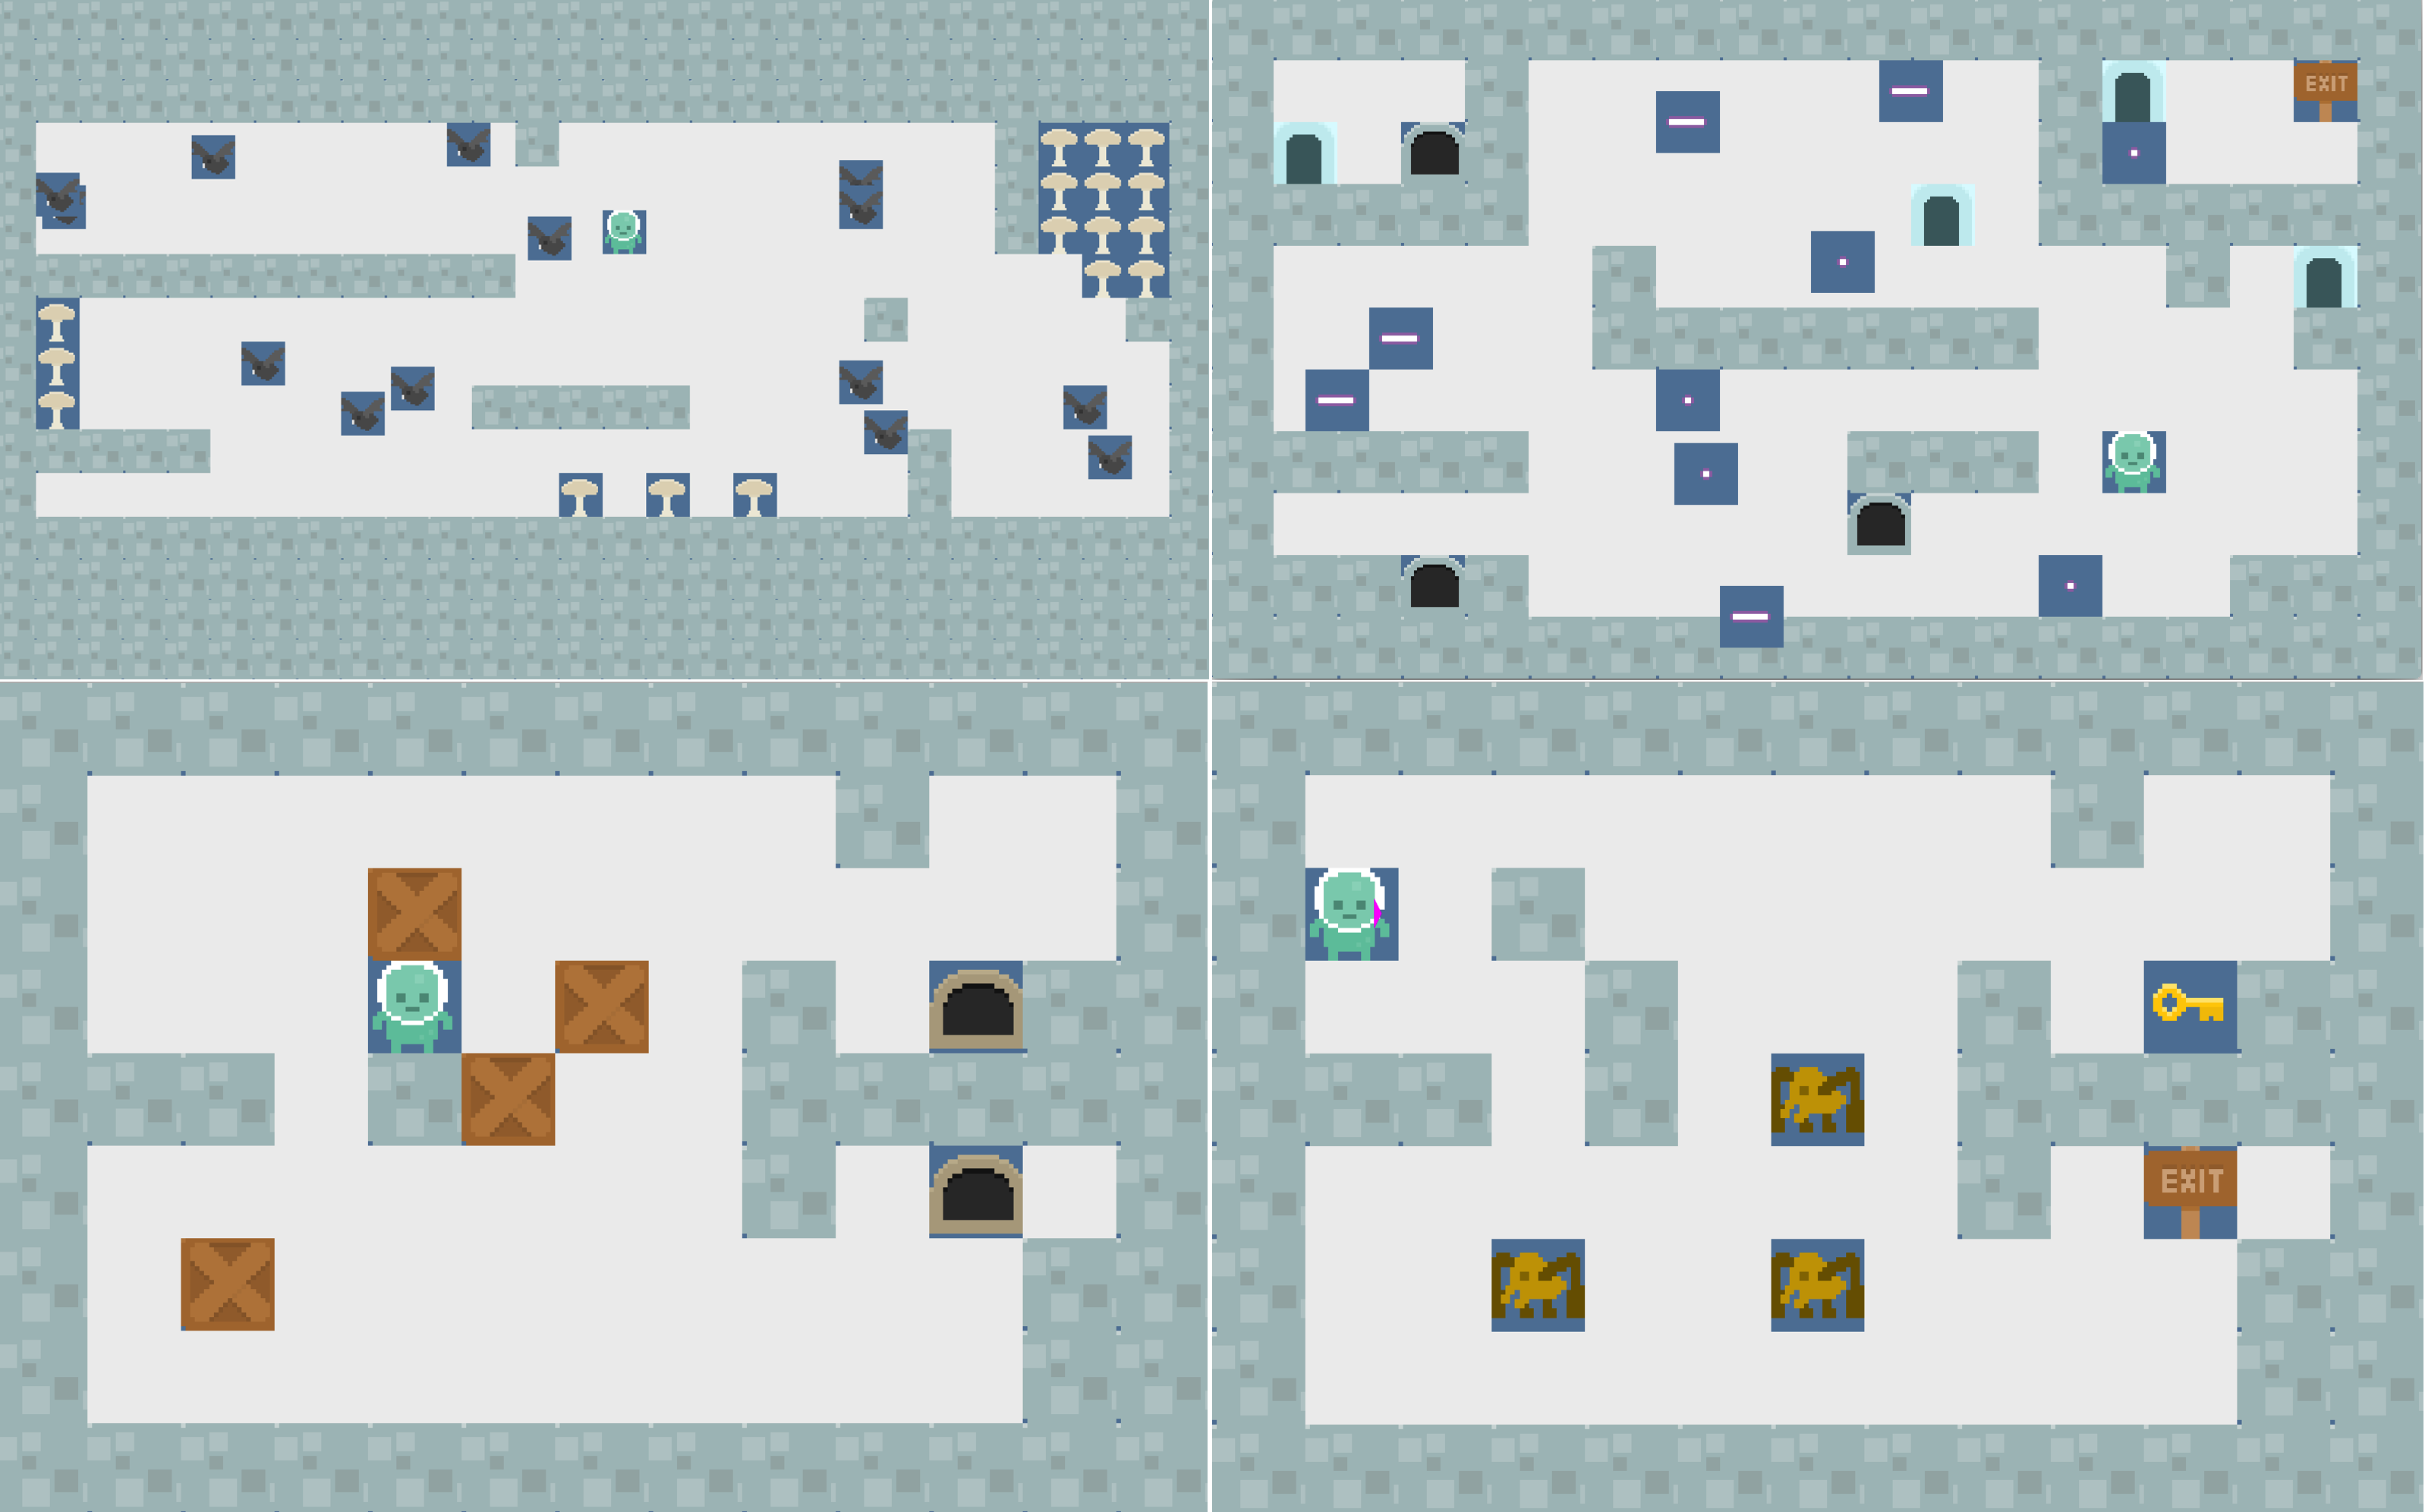
\includegraphics[width=1.8\columnwidth]{img/games}
\end{center}
\caption{Four of the ten training set games: from top to bottom, left to right, \textit{Butterflies}, \textit{Portals}, \textit{Sokoban} and \textit{Zelda}.}
\label{fig:games}
\end{figure*}



\section{Approaches} \label{sec:approaches}

\subsection{Learning Algorithms}
As stated in the introduction, we coupled two different kinds of function approximators with two different exploration policies, and evolved their weights. Assuming input features $\phi$ and a set of actions $A$ (with each action $a \in A$), we evolved a set of weights for each action $w_a$:
\begin{itemize}
\item $p^{linear}_a = w_a^0 \cdot \phi$ for the linear function approximator.
\item $p^{nn}_a = w_a^0 \cdot \max { (w_1 \cdot \phi, 0) } $ for the rectifier neural network~\cite{glorot2011deep}.
\end{itemize}
The types of exploration used are \textit{Softmax} and $\epsilon$-\textit{greedy}. We normalise all inputs on the function approximators between -1 and 1. Notice that the output layer of weights $w_a^0$ for the neural network approximator is the same for all actions and set to $20$ (i.e., the total number of hidden neurons). The number of neurons used is mostly an ad-hoc choice, however it is small enough to be evolved online. 

Using $p_a$ we define two different policies:

\begin{itemize}
\item $\pi^\epsilon(\phi,a) = \twopartdefo{ 1-\epsilon + \epsilon/|A| }{ a = \argmax\limits_{a \in A}  p_a}{\epsilon/|A|}$
\item $\pi^{softmax}(\phi,a) = e^{p_a}/ \sum\limits_{b \in A} p_b $
\end{itemize}

These two policies were chosen because of their ease of implementation and their popularity - they are the two most common exploration policies. For all our experiments, $\epsilon$ is always set to $0.1$. All four possible combinations of polices and function approximators are used in the experiments. Training the function approximators involves learning the weights $w$. We use Separable Natural Evolution Strategies (S-NES) for this~\cite{schaul2011high}. Since we used at least $7$ features for each action, and GVG-AI supports $4$ actions, we would have a $28$ dimensional problem for the linear approximator and a $220$ dimensional problem for the neural network appoximator at the very minimum. Since S-NES is an evolution strategy that follows the natural gradient (which can be seen as a gradient that uses KL-divergence as a measure of distance instead of euclidean distance). It assumes that the search parameters come from a multi-variate Gaussian distribution and tries to adapt the Gaussian's mean and covariance-matrix using the natural gradient. The natural gradient allows for information on the uncertainty of the estimates to be incorporated in the gradient search, as well as making the search invariant to transformation. A further transformation on the fitness structure of the problem also takes place; using a population of samples, the fitness is transformed to $[0,1]$ using a ranking scheme, which makes the algorithm invariant to transformations of the target function as long as these transformations do not impact ranking order. The ``Separable'' element of the algorithm used here refers to adapting only the diagonal elements of the covariance matrix. This speeds up learning significantly, allowing the S-NES to scale linearly to problems of arbitrary size (instead of quadratically), making the algorithm practical for our situation. For a more detailed explanation of the algorithm, the reader is referred to~\cite{schaul2011high}. 

\subsection{Game features} \label{ssec:feat}

All algorithms employed in this experimental study use the same set of features $\phi$ for learning. These features are extracted from the game state, which is received in the format explained in Section~\ref{ssec:framework} and Table~\ref{tab:inf}. The features employed in this research are all of a numeric nature, and they are detailed next:

\begin{mitems}
\item Game score.
\item Game tick.
\item Game winner ($-1$ if game is still ongoing, $0$ if the player lost and $1$ if the player won).
\item Game over ($1$ if game is over, $0$ otherwise).
\item Resources: list of the amount of resources owned by the avatar\footnote{In order to have a fixed number of features, the length of this list is set to $5$ (the number of avatar resources can vary from game to game, from none to $N$ types).}.
\item List with the Euclidean distances to the closest sprite of each type. 
\item Speed of the avatar.
\end{mitems}

Note that the features are common in all games and are very general (i.e. they do not change from game to game). It is possible however that one might not want to use any features - there is indeed an option and one could use the underlying object structure directly. 



\section{Experiments} \label{sec:exp}

The algorithms proposed in the previous section have been tested in the games described previously in Section~\ref{ssec:games}. For each one of the $10$ present games, the first available level has been used for a learning process where each algorithm played $1000$ consecutive times. For each game, $50$ experiments where run, and the average of the progression of the score is plotted in Figures~\ref{fig:results1} and~\ref{fig:results2}. 

\newcommand*{\lefig}{0.43}%

\begin{figure*}[!t]
	\begin{center}
%	\vspace{-3mm}
\begin{subfigure} {\lefig\textwidth}
	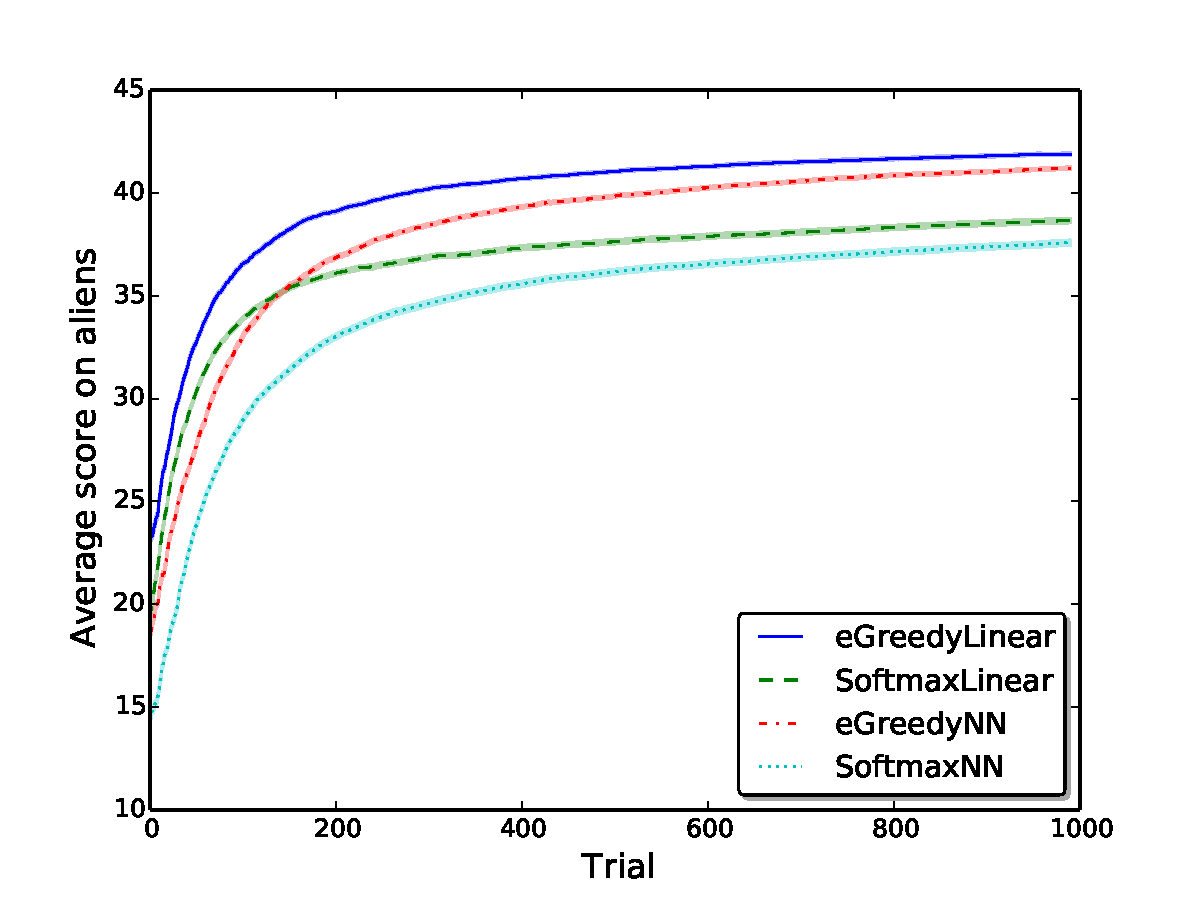
\includegraphics[width =\textwidth]{img/aliens_scores}
  \caption{Aliens}
\end{subfigure}\begin{subfigure} {\lefig\textwidth}
	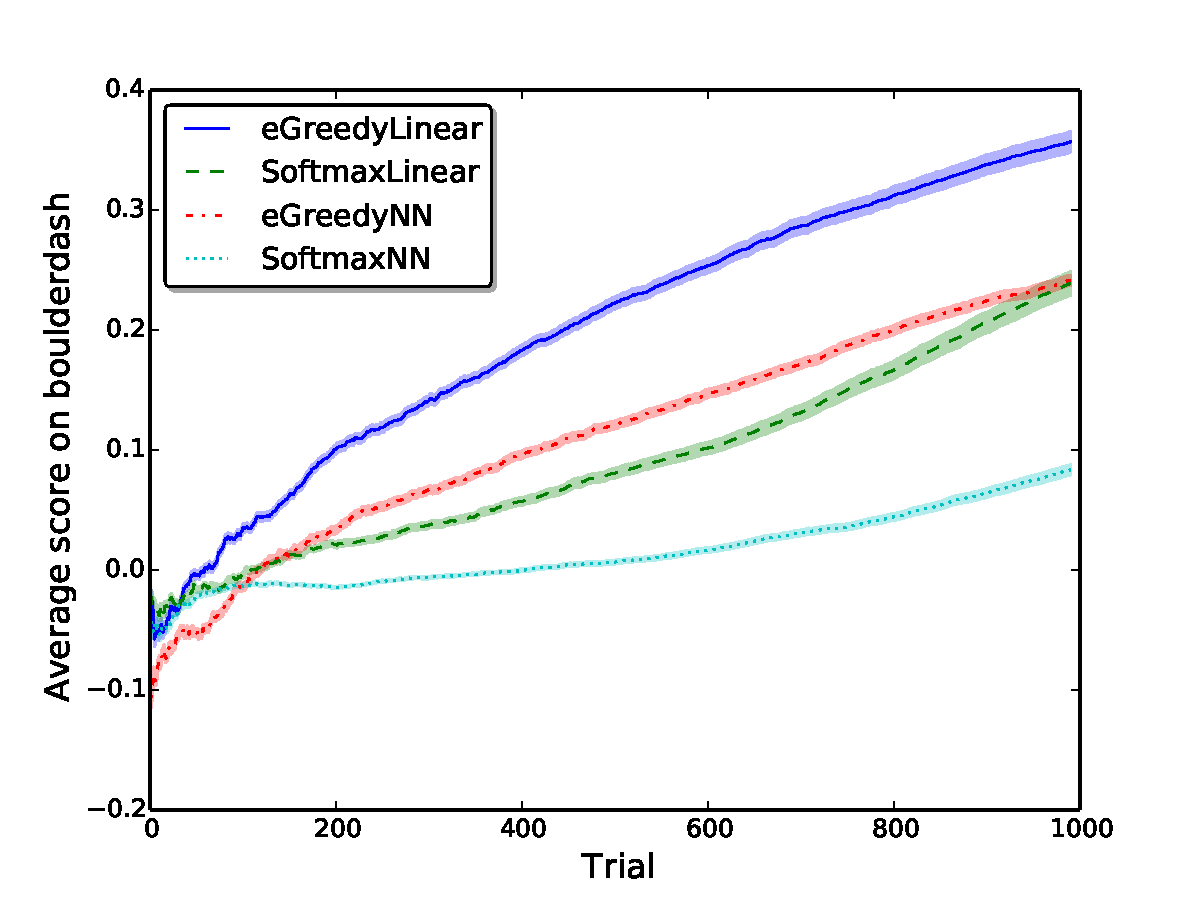
\includegraphics[width = \textwidth]{img/boulderdash_scores}
  \caption{Boulderdash}
\end{subfigure}
%	\vspace{-3.5mm}

\begin{subfigure} {\lefig\textwidth}
	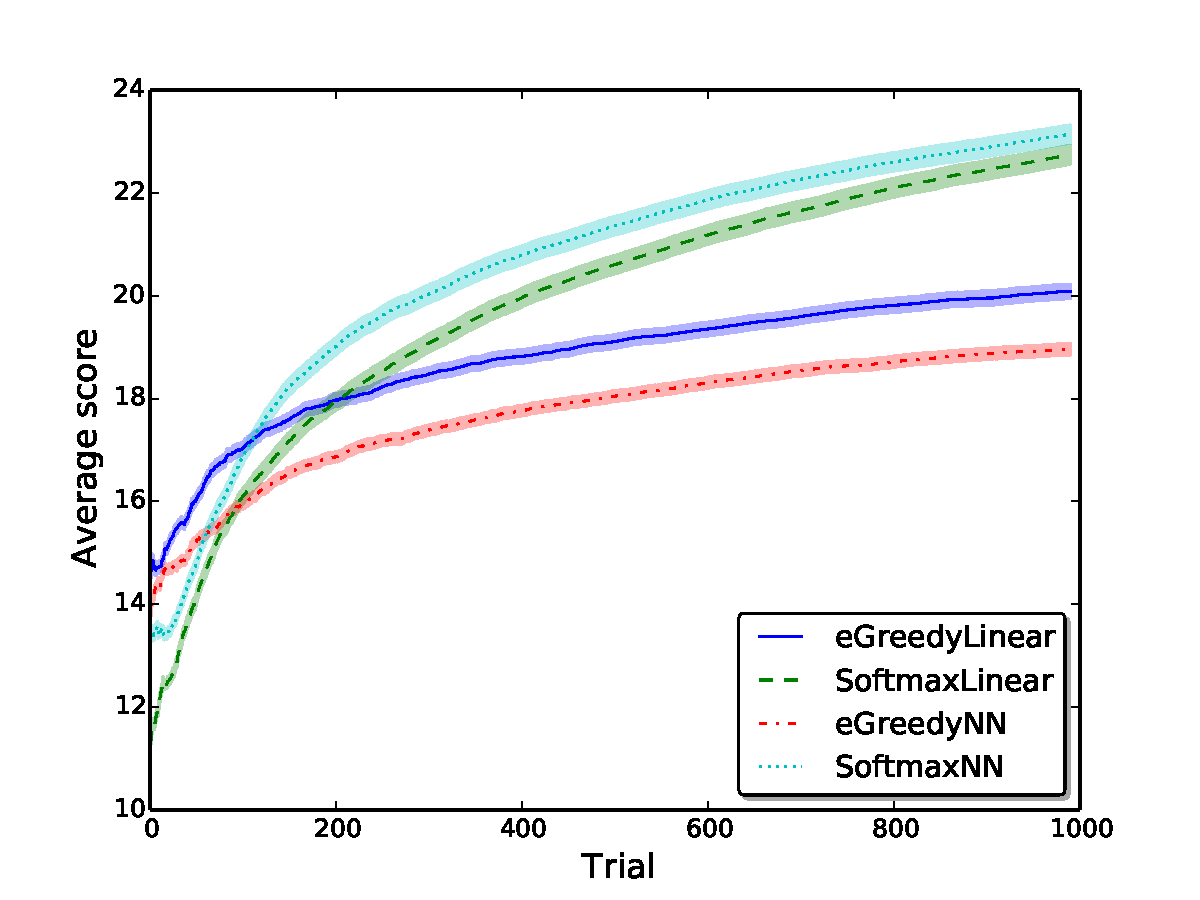
\includegraphics[width = \textwidth]{img/butterflies_scores}
  \caption{Butterflies}
\end{subfigure}\begin{subfigure} {\lefig\textwidth}
	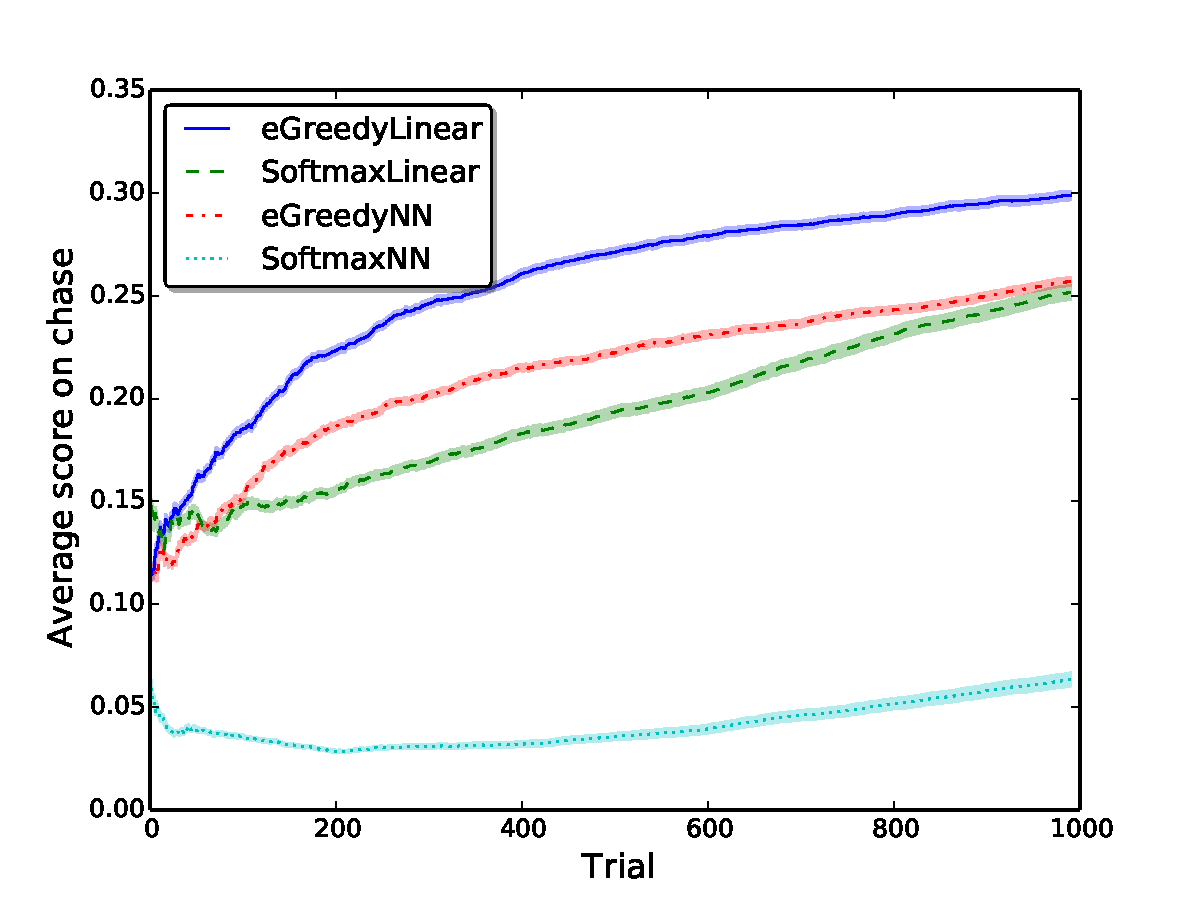
\includegraphics[width = \textwidth]{img/chase_scores}
  \caption{Chase}
  \end{subfigure}
%	\vspace{-3.5mm}

\begin{subfigure} {\lefig\textwidth}
	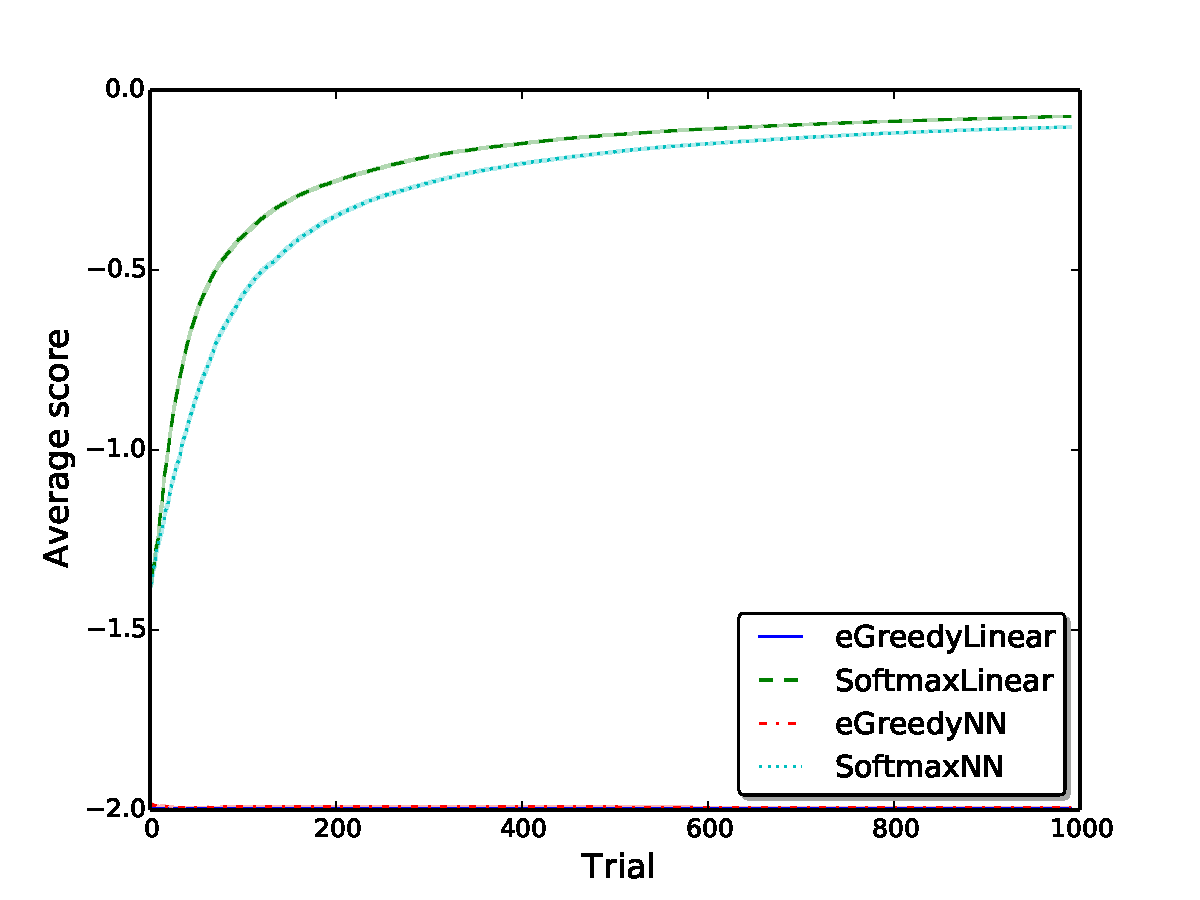
\includegraphics[width = \textwidth]{img/frogs_scores}
  \caption{Frogs}
\end{subfigure}\begin{subfigure} {\lefig\textwidth}
	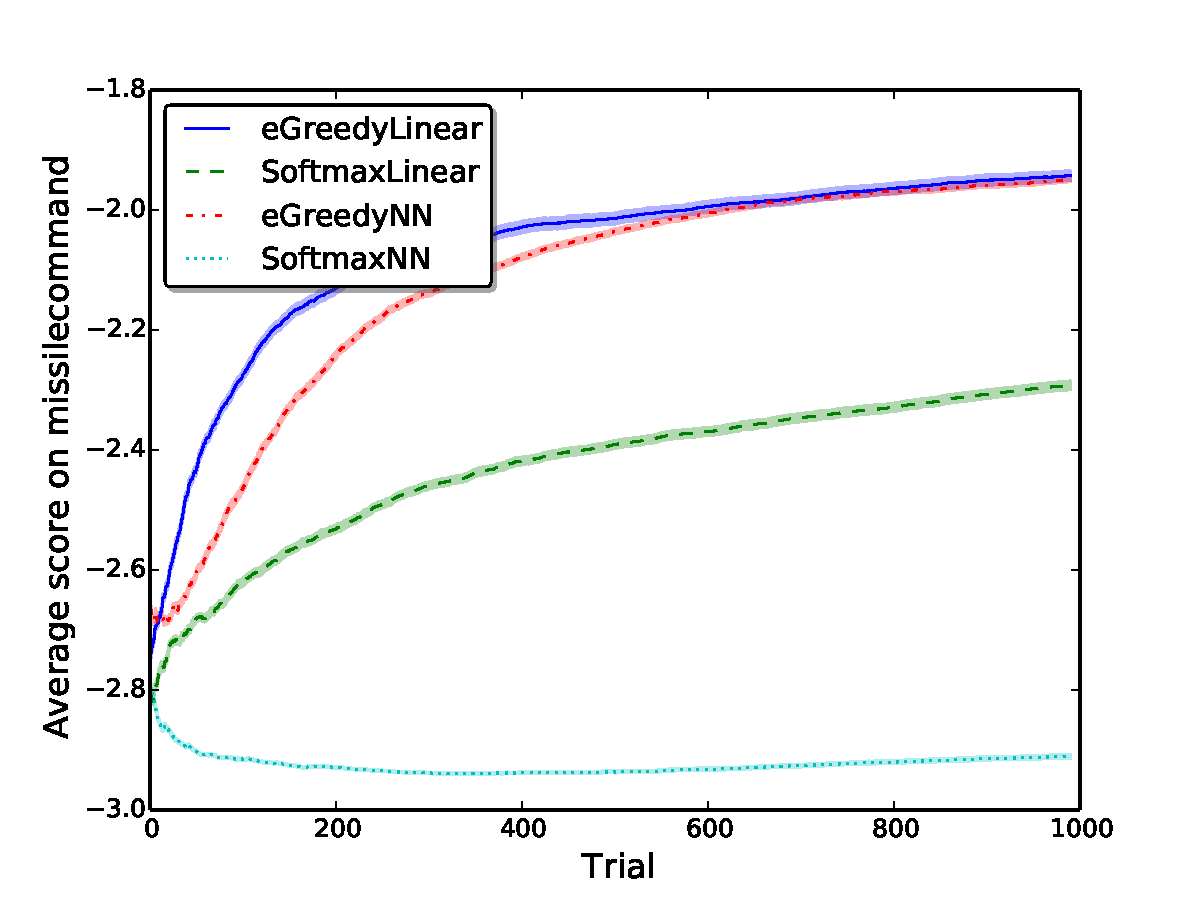
\includegraphics[width = \textwidth]{img/missilecommand_scores}  
  \caption{Missile Command}
\end{subfigure}
%	\vspace{-1mm}
	\caption{Progression of the average score during $1000$ trials. Horizontal axis denotes the trial, while the vertical axis shows the average score. Shadowed area indicates the standard error of the measure. From left to right, top to bottom, the games are \textit{Aliens}, \textit{Boulderdash}, \textit{Butterflies}, \textit{Chase}, \textit{Frogs} and \textit{MissileCommand}.}
	\label{fig:results1}
	\end{center}
\end{figure*}


\begin{figure*}[!t]
	\begin{center}
%	\vspace{-3mm}

%	\vspace{-3.5mm}
\begin{subfigure} {\lefig\textwidth}
	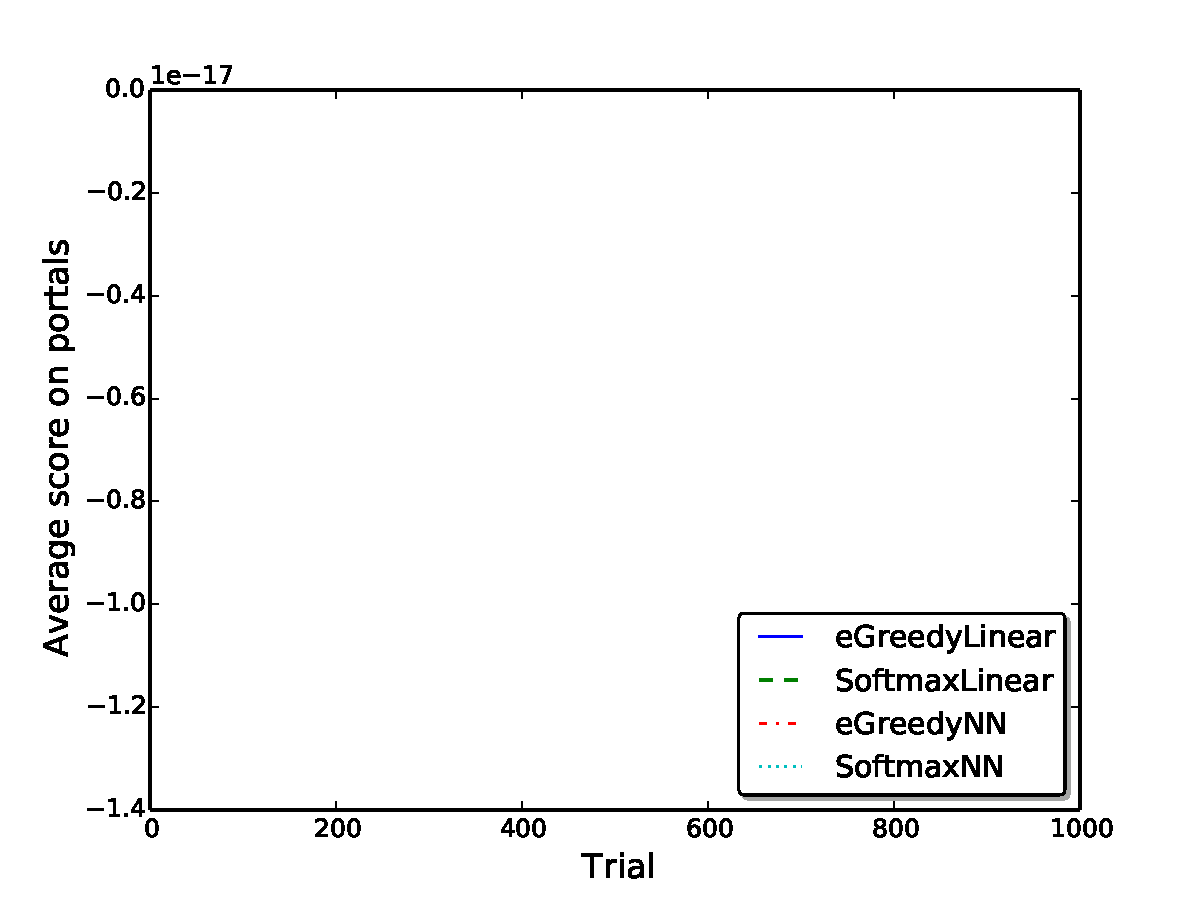
\includegraphics[width = \textwidth]{img/portals_scores}
  \caption{Portals}
\end{subfigure}\begin{subfigure} {\lefig\textwidth}
	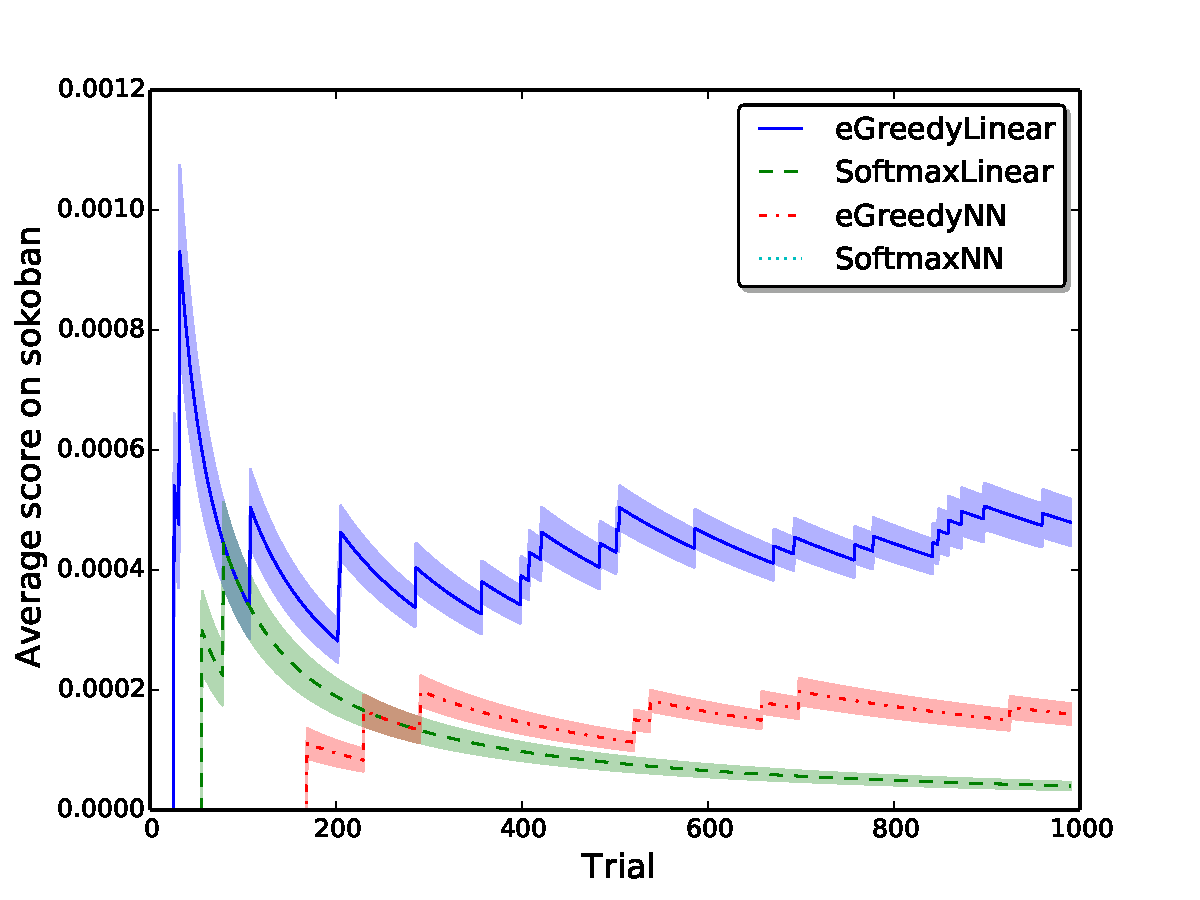
\includegraphics[width = \textwidth]{img/sokoban_scores}
  \caption{Sokoban}
\end{subfigure}

\begin{subfigure} {\lefig\textwidth}
	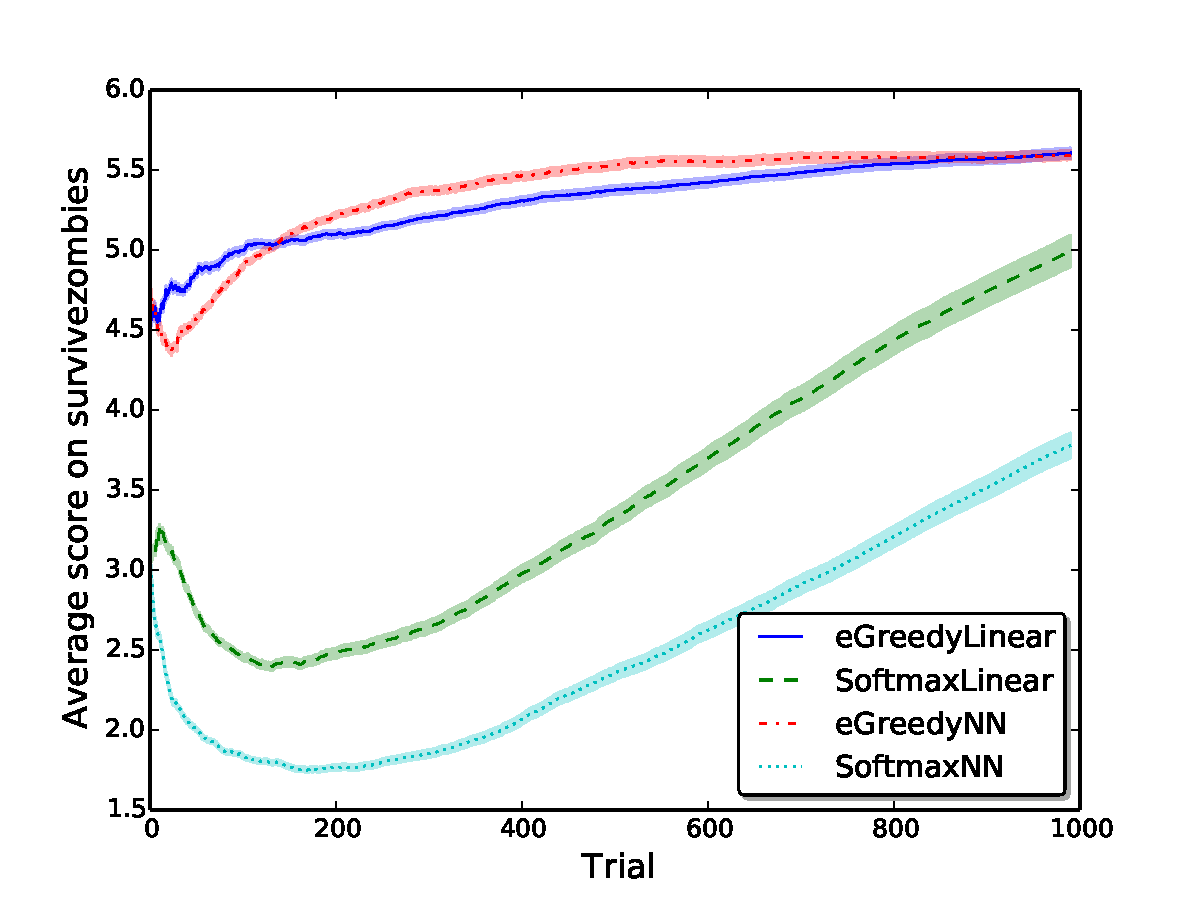
\includegraphics[width = \textwidth]{img/survivezombies_scores}
  \caption{Survival Zombies}
\end{subfigure}\begin{subfigure} {\lefig\textwidth}
	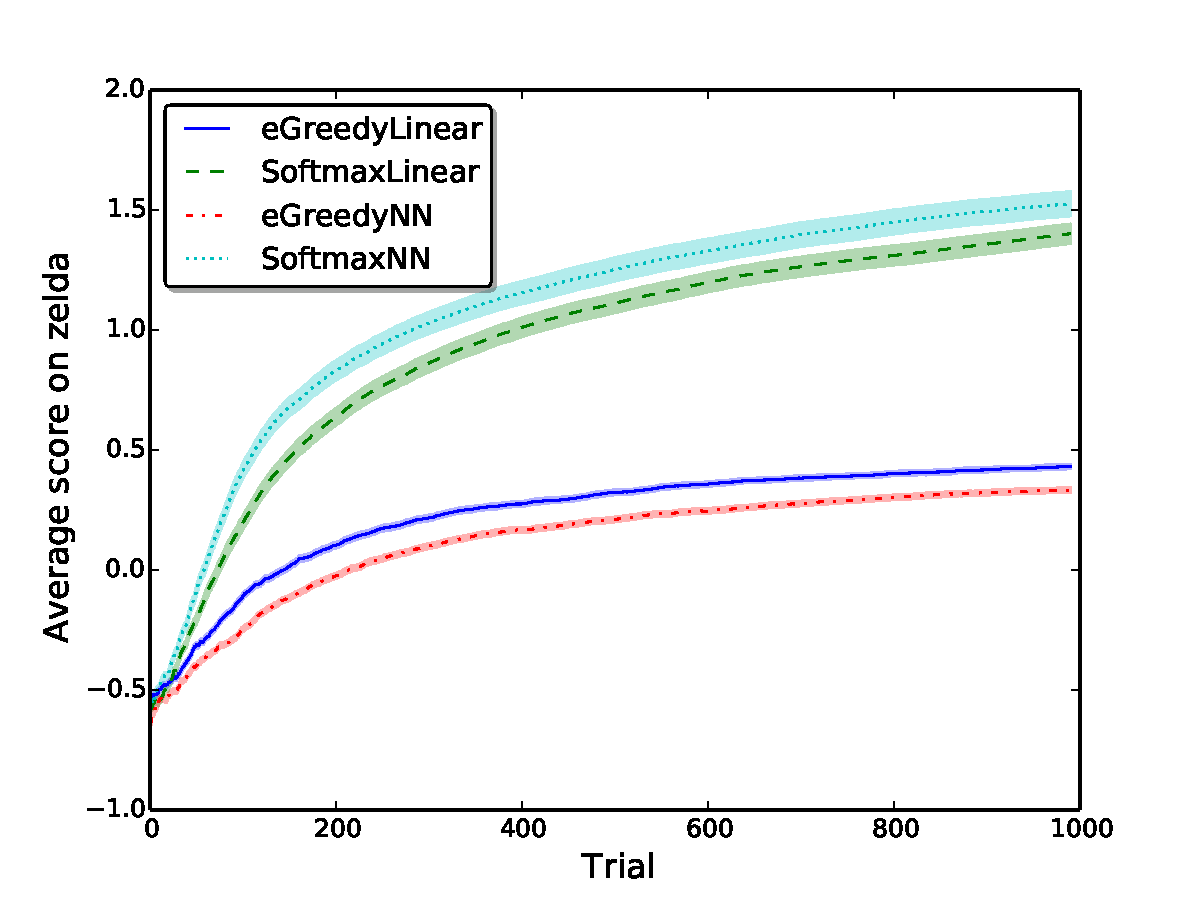
\includegraphics[width = \textwidth]{img/zelda_scores}
  \caption{Zelda}
\end{subfigure}

%	\vspace{-1mm}
	\caption{Progression of the average score during $1000$ trials. Horizontal axis denotes the trial, while vertical axis shows the average score. Shadowed area indicates the standard error of the measure. From left to right, top to bottom, the games are \textit{Portals}, \textit{Sokoban}, \textit{SurviveZombies} and \textit{Zelda}.}
	\label{fig:results2}
	\end{center}
\end{figure*}

These figures show the average of score, including the standard error (shadowed area), as it progresses with the number of matches, for each one of the games played. The first aspect to realize is that learning can be appreciated in $8$ out of the $10$ games employed in the experimental study. It is not possible to declare any of the algorithms as an overall best option, as it generally depends on the game played. 

It seems clear that in some games (such as \textit{Aliens}, \textit{MissileCommand} or \textit{SurviveZombies}) the algorithms with an $\epsilon$-\textit{greedy} policy learn better, while in others (such as \textit{Frogs} or \textit{Zelda}) it is the algorithms with a \textit{Softmax} policy the ones with a better performance. For instance, in the game \textit{Frogs}, $\epsilon$-\textit{greedy} algorithms are not able to survive (a score of $-2$ reflects that the player is killed by a truck), while \textit{Softmax}  approaches are capable of learning how to avoid these. Regarding the approximations used, even when the difference is small, the results suggest that the linear approximator works better than the neural network, for both policies tested and most of the games. A possible explanation for this is that the neural network operates in a larger search space, which can potentially inhibit its learning capabilities in the short term.

The cases were learning cannot be achieved by any of the algorithms tested here happen in the games \textit{Portals} (where the score is $0$ through the whole process) and \textit{Sokoban} (with an interesting jagged curve). The low performance of all algorithms in these two games can be due to different reasons.

In the case of \textit{Portals}, the game requires a long sequence of movements (traversing portals) before reaching the goal, which is the only moment where the agent receives positive feedback. As reaching the exit is extremely unlikely, the flat landscape of rewards inhibits the agent from learning how to score points in the game. Interestingly, the hazards in the game that kill the player are well avoided in general. The results show that the time spent in the game (a measure not depicted here for clarity) is close to $60$ and $100\%$ of the maximum time allowed (for algorithms with $\epsilon$-\textit{greedy} and \textit{Softmax} policies, respectively). This means that the algorithms, specially the ones with a \textit{Softmax} policy, are able to learn very quickly how to survive in this game, albeit ending with a score of $0$.

An explanation for the strange results on \textit{Sokoban} may be related to the features used for learning. In this game, score is awarded when a box is introduced into a hole in the level. With the features extracted from the game state (see Section~\ref{ssec:feat}), this can be related to minimizing distances between the avatar and the closest box, and between the avatar and the closest hole, both at the same time. The problem is that these minimizations must happen simultaneously, having the avatar pushing in the right direction and with the presence of a hole at the other side of the box. These situations happen rarely, and it is reflected in this game's plot with picks along the curve. As the features only allow the algorithms to determine distances (and not the supplementary needed requirements), they are not able to learn properly and their performance decreases. The game of \textit{Sokoban} has been traditionally one of the most difficult ones from the GVGAI framework and competition~\cite{Perez2015}, as it requires long term plans for its completion.

It is also worthwhile highlighting that in some games, after the $1000$ matches, the improvement on the score average has not stopped, which suggests that better results can be found with longer execution trials.


\section{Conclusions} \label{sec:conc}

This paper shows a first comparison of different policies ($\epsilon$-\textit{greedy} and \textit{Softmax}) and function approximators, using an evolutionary algorithm (S-NES) as a learning scheme. The objective of the agents that implement these algorithms is to learn how to maximize the score in $10$ different games, without the help of any domain specific-heuristic, something that was (at least partially) achieved. Additionally, all these games have different characteristics, which allows us to examine under what conditions learning is performed better. What we have shown is that under most scenarios, using a $\epsilon$-\textit{greedy} algorithm coupled with a linear function approximator is the fastest, surest way to get reasonably good results. This is not that unintuitive, as there are fewer variables to learn and a more ``greedy'' version of learning can take place, compared to softmax. 

In this study, the algorithms tested are able to learn in most of the games tested. In particular, linear function approximators seem to perform best in this setup, although results may vary from game to game, with different algorithms providing a distinct performance. Results also suggest that games requiring a long term plan (such as \textit{Sokoban} or \textit{Portals}) may require a different approach for getting learning to work, one that might include substantial exploration, as the lack of any learning signal proves fatal. 

Although the robustness of evolutionary computation is commendable, it might be worth attacking the same problems using more traditional, gradient-based approaches (e.g, Monte Carlo methods, SARSA/Q Learning). This would allow for the training of deeper networks which could possibly help. This could be coupled without using features at all, but rather using the raw bitplanes as input. It is also obvious that more training would be very beneficial for a number of games. 

Finally, an important point to make here is that effectively testing and learning are happening on the same levels. Including more levels (and also increasing the size of the game set used for experiments) for each game will bring further details about how general the algorithms tested in this research are, and will allow for a deeper analysis on their learning abilities in the domain of General Video Game Playing. This highlights the  difficulty of the domain where one has to learn extremely quickly, without much access to heuristics and/or an environmental model. 


% use section* for acknowledgement
 

\bibliographystyle{IEEEtran} 
\bibliography{biblio}


% that's all folks
\end{document}


